% Made up for the tikra benchmark.
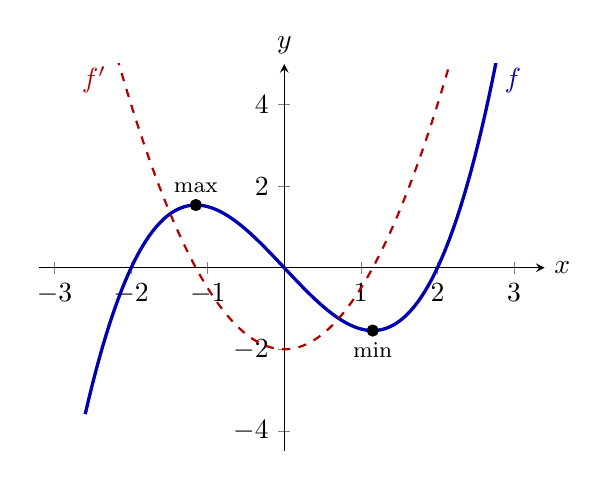
\begin{tikzpicture}
\begin{axis}[axis lines=center, xmin=-3.2, xmax=3.4, ymin=-4.5, ymax=5,
    xlabel=$x$, ylabel=$y$, xtick={-3,...,3}, ytick={-4,-2,2,4},
    every axis x label/.style={at={(ticklabel* cs:1)}, anchor=west},
    every axis y label/.style={at={(ticklabel* cs:1)}, anchor=south},
    width=8cm, height=6.5cm, samples=120]
  \addplot[very thick, blue!70!black, domain=-2.6:2.9] {0.5*x^3 - 2*x};
  \addplot[thick, red!70!black, dashed, domain=-3:3] {1.5*x^2 - 2};
  \addplot[only marks, mark=*, mark size=2pt, black] coordinates {
    (-1.1547,1.5396) (1.1547,-1.5396)};
  \node[above, font=\footnotesize] at (axis cs:-1.1547,1.6) {max};
  \node[below, font=\footnotesize] at (axis cs:1.1547,-1.6) {min};
  \node[blue!70!black, right] at (axis cs:2.75,4.6) {$f$};
  \node[red!70!black, left] at (axis cs:-2.2,4.6) {$f'$};
\end{axis}
\end{tikzpicture}
